\chapter{Results}

\section{Generation Time}

\begin{figure}[h]
	\centering
	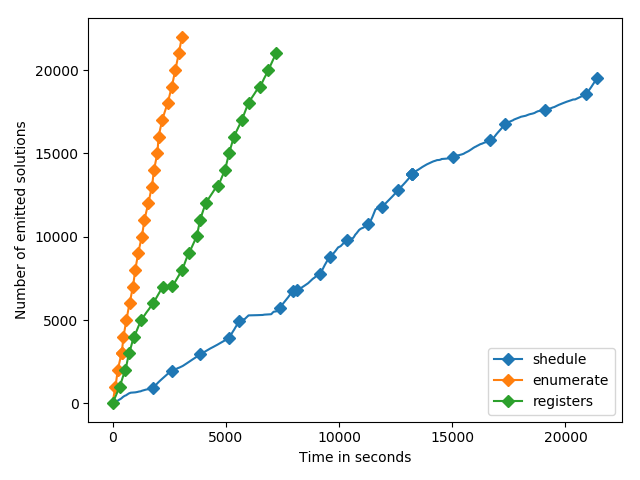
\includegraphics[width=\textwidth,height=0.5\textheight]{results/figures/generator_time}
	\caption{The execution time of the code generator at sampling rate 1000 (i.e 1000000 solutions for every function). Each marker represents the finished generation of a function. The markers are ordered so that the nth marker on every line represents the same function. Total time is annotated as hours and minutes.}
	\label{fig:time}
\end{figure}

The execution times of the constraint solver at sampling rate 1000 are shown in Figure
\ref{fig:time}. Each marker represents the completed generation of a function. I.e for each
marker 1000000 (one million) solutions have been explored. For a few functions fewer than
1000 solutions were found (for a complete breakdown see appendix \ref{appendix:function_names}).

While the total execution time is daunting, it does represent about 23 million solutions
found (but only 23000 emitted). The enumerate strategy is fairly quick; 51 minutes for one
million solutions of every function means that on average, one solution was found every
139ns. The same number for registers and schedule is 343ns and 1095ns respectively. To
mitigate the impact of a long execution time the solutions can be emitted directly when
found.

disUnison does not use the same search heuristics as the base Unison model. The disUnison
search heuristics makes implementation easier at the potential cost of execution time. The
problem with optimizing the branching and search heuristics of the model is that the
performance impact will largely have to be determined empirically. Supposedly, the optimal
search heuristic for the registers strategy would not be the same as the optimal search
heuristic for the schedule strategy.

\section{Cost}

The estimated cost of each program is shown in Figure \ref{fig:cost}. The dotted red line
shows the cost of the LLVM solution when calculated in the same manner.

\begin{figure}[h]
	\centering
	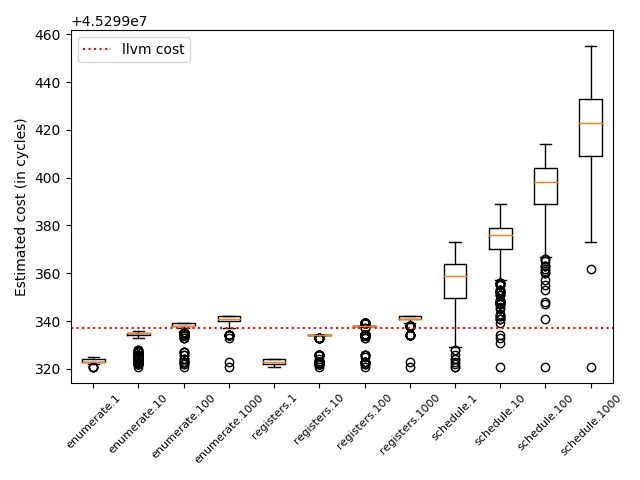
\includegraphics[width=\textwidth,height=0.5\textheight]{results/figures/cost}
	\caption{The cost distributions for every strategy and sampling rate. The cost of the LLVM solution is included for reference.}
	\label{fig:cost}
\end{figure}

All strategies perform better for lower sampling rates. As described in section
\ref{sec:performance}, this is expected. Enumerate and registers perform equally well and
for sampling sizes of 1 and 10 they have a lower cost than the LLVM solution. The schedule
strategy seems to incur a slight overhead compared to the LLVM solution for all sampling
rates.

\begin{table}[h]
		\centering
		\noindent\makebox[\textwidth]{%
			\begin{tabular}{rrrr}
\hline
   Sampling Rate &   Est. Cost (cycles) &   Difference (cycles) &   Overhead (\textperthousand) \\
\hline
               1 &             45299359 &                    22 &                      0.000486 \\
              10 &             45299376 &                    39 &                      0.000861 \\
             100 &             45299398 &                    61 &                      0.001347 \\
            1000 &             45299423 &                    86 &                      0.001898 \\
\hline
\end{tabular}
		}
		\caption{The cost of the different sampling rates for the schedule strategy compared to the LLVM solution.%
		The difference column is the difference between the median cost of the sampling rate and the cost of the LLVM solution.}
		\label{table:sched_cost}
\end{table}

Table \ref{table:sched_cost} shows the cost difference between the different sampling
rates for the schedule strategy compared to the cost of the LLVM program. The overhead of
the schedule strategy is negligible (note that the overhead column shows per mille). All
sampling rates have versions with a lower cost than the LLVM solution so if only a few
versions are necessary there is potential to limit the constraint solver to only find
those with lower cost than LLVM.

Interesting to note is that all strategies and sampling rates have found a solution with
an equally low cost. This is presumably the very first solution found; When no strategy
related constraints have been posted yet. Thanks to the search heuristic, where lower cost
solutions are explored first, this is also the optimal cost.

\section{Surviving Gadgets}

\begin{figure}[htp]
	\centering
	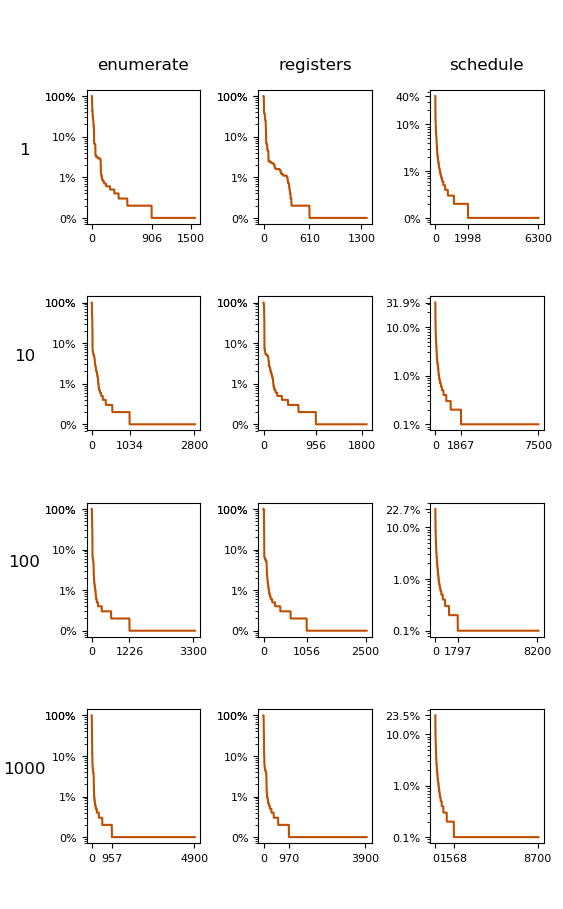
\includegraphics[width=\textwidth,height=\textheight]{results/figures/gadgets}
	\caption{The ratio of occurrence for each gadget broken down by strategy and sampling rate.
Each dot shows the occurrence ratio for one particular gadget. The data is sorted to allow
	for a better overview.}
	\label{fig:gadgets}
\end{figure}

Figure \ref{fig:gadgets} shows the occurrence ratio of each gadget for the different
strategies and sampling rates. The x-axis shows a gadget id and there is no definitive
correlation between the gadgets across strategies and sampling rates. I.e gadget 0 for the
enumerate strategy at sampling rate 1 is not necessarily the same gadget 0 as the registers
strategy at sampling rate 10.

As seen in figure \ref{fig:gadgets}, neither the enumeration nor the registers strategy
were particularly effective at breaking gadgets for any sampling rate. There is a slight
improvement for higher sampling rates but it is not particularly impressive even at
sampling rate 1000. There are still many gadgets that survives across a large percentage of
versions. The schedule strategy, however, performed well with no gadget being present
in even 50\% of all versions for the lowest sampling rate and for sampling rate 1000
about 82\% of gadgets only appear in one version.

Unfortunately, due to the shortcomings of the experiment this results is not comparable to
the ones presented in other literature. However, it does hint at the potential gadget-
breaking properties of each strategy. Enumerate and registers show decent potential and the
schedule strategy shows great potential but it would have to be verified on a proper
executable for the x86-64 architecture.

\section{Conclusion and Future Work}

The core of the disUnison model, the three strategies, are implemented in just a handful
lines of code and, thanks to being an extension of the Unison model, there is never a risk
of breaking the functionality of the generated code. This is not to say that every
diversification strategy allows for proper executable code to be generated, but thanks to
the nature of constraint solving the result will either be all possible solutions
(given enough execution time) or a proof that no solution, and thus no proper executable,
exists.

Regardless of what the selection of strategies may indicate the possibilities for
diversification are far broader than when approaching the problem in terms of register
allocation and instruction scheduling as separate procedures. It is important to keep in
mind that more unorthodox strategies that exploit the combined approach might be even
more performant. As mentioned in \ref{sec:strategies} the Unison model consists of more
variables than the 4 explored in this experiment, all of which offers potential for
diversity.

By exploring lower cost solutions first and applying tiny, incremental changes between
solutions the resulting code is relatively performant. There is also an opportunity to
add constraints to the model that steers this cost in some direction. By not randomizing
we have full control of the process and can limit the resulting code in whatever way is
appropriate.

For a more proper comparison of the systematic approach tests would have to be repeated
targeting the x86-64 architecture. As mentioned in Section \ref{sec:arch} Unison in its
current state does not support the x86-64 architecture. If or when Unison or a similar
tool implements support for the x86-64 architecture, the experiment would have be repeated
on that platform to test whether or not the strategies are equally performant.

Another shortcoming is the difficulty of compiling a large program even without applying
diversification strategies. Most of the functions of 433.milc were too large to find even
one solution (when searching for about one hour). This is an obvious problem for any
practical purpose of the systematic approach. One solution to this problem is to modify
the search heuristics of the disUnison model even further. Unfortunately it would be
difficult, if not impossible, to find an optimal, generally-applicable search strategy.

Using a constraint solver to generate diverse binaries is an attractive approach given
the ease of implementation and the quality of the generated code. The resulting population
of diversified programs shows that the systematic approach has great potential at breaking
gadgets. However, the shortcomings of the experiment and the tool are a testament to the
future work required.
